% This file was converted to LaTeX by Writer2LaTeX ver. 1.0.2
% see http://writer2latex.sourceforge.net for more info
\documentclass[twoside,letterpaper]{article}
\usepackage[latin1]{inputenc}
\usepackage[T1]{fontenc}
\usepackage[english]{babel}
\usepackage{amsmath}
\usepackage{amssymb,amsfonts,textcomp}
\usepackage{color}
\usepackage{array}
\newcolumntype{M}[1]{>{\centering\arraybackslash}m{#1}}
\usepackage{supertabular}
\usepackage{hhline}
\usepackage{hyperref}
\usepackage{float}
\hypersetup{pdftex, colorlinks=true, linkcolor=blue, citecolor=blue, filecolor=blue, urlcolor=blue, pdftitle=SOFTWARE DESIGN DOCUMENT (SDD), pdfauthor=Shaylyn Adams}
\usepackage[pdftex]{graphicx}
\usepackage{subcaption}
% Outline numbering
\setcounter{secnumdepth}{5}
\renewcommand\thesection{\arabic{section}}
\renewcommand\thesubsection{\arabic{section}.\arabic{subsection}}
\renewcommand\thesubsubsection{\arabic{section}.\arabic{subsection}.\arabic{subsubsection}}
\renewcommand\theparagraph{\arabic{section}.\arabic{subsection}.\arabic{subsubsection}.\arabic{paragraph}}
\renewcommand\thesubparagraph{\arabic{section}.\arabic{subsection}.\arabic{subsubsection}.\arabic{paragraph}.\arabic{subparagraph}}
\makeatletter
\newcommand\arraybslash{\let\\\@arraycr}
\makeatother
% Page layout (geometry)
\setlength\voffset{-1in}
\setlength\hoffset{-1in}
\setlength\topmargin{0.5in}
\setlength\oddsidemargin{1in}
\setlength\evensidemargin{1in}
\setlength\textheight{8.278in}
\setlength\textwidth{6.5in}
\setlength\footskip{0.561in}
\setlength\headheight{0.5in}
\setlength\headsep{0.461in}
% Footnote rule
\setlength{\skip\footins}{0.0469in}
\renewcommand\footnoterule{\vspace*{-0.0071in}\setlength\leftskip{0pt}\setlength\rightskip{0pt plus 1fil}\noindent\textcolor{black}{\rule{0.25\columnwidth}{0.0071in}}\vspace*{0.0398in}}
% Pages styles
\makeatletter
\newcommand\ps@Standard{
  \renewcommand\@oddhead{\selectlanguage{english}\rmfamily\color{black} University of Massachusetts CICS \hfill \hfill Health-e}
  \renewcommand\@evenhead{\@oddhead}
  \renewcommand\@oddfoot{\foreignlanguage{english}{\textcolor{black}{SDD Page }}\foreignlanguage{english}{\textcolor{black}{\thepage{}}}}
  \renewcommand\@evenfoot{\@oddfoot}
  \renewcommand\thepage{\arabic{page}}
}
\newcommand\ps@Convertviii{
  \renewcommand\@oddhead{}
  \renewcommand\@evenhead{\@oddhead}
  \renewcommand\@oddfoot{}
  \renewcommand\@evenfoot{\@oddfoot}
  \renewcommand\thepage{\arabic{page}}
}
\newcommand\ps@Convertvii{
  \renewcommand\@oddhead{}
  \renewcommand\@evenhead{\@oddhead}
  \renewcommand\@oddfoot{}
  \renewcommand\@evenfoot{\@oddfoot}
  \renewcommand\thepage{\arabic{page}}
}
\newcommand\ps@Convertvi{
  \renewcommand\@oddhead{}
  \renewcommand\@evenhead{\@oddhead}
  \renewcommand\@oddfoot{}
  \renewcommand\@evenfoot{\@oddfoot}
  \renewcommand\thepage{\arabic{page}}
}
\newcommand\ps@Convertv{
  \renewcommand\@oddhead{}
  \renewcommand\@evenhead{\@oddhead}
  \renewcommand\@oddfoot{}
  \renewcommand\@evenfoot{\@oddfoot}
  \renewcommand\thepage{\arabic{page}}
}
\newcommand\ps@Convertiv{
  \renewcommand\@oddhead{}
  \renewcommand\@evenhead{\@oddhead}
  \renewcommand\@oddfoot{}
  \renewcommand\@evenfoot{\@oddfoot}
  \renewcommand\thepage{\arabic{page}}
}
\newcommand\ps@Convertii{
  \renewcommand\@oddhead{}
  \renewcommand\@evenhead{\@oddhead}
  \renewcommand\@oddfoot{}
  \renewcommand\@evenfoot{\@oddfoot}
  \renewcommand\thepage{\arabic{page}}
}
\newcommand\ps@FirstPage{
  \renewcommand\@oddhead{}
  \renewcommand\@evenhead{\@oddhead}
  \renewcommand\@oddfoot{}
  \renewcommand\@evenfoot{\@oddfoot}
  \renewcommand\thepage{\arabic{page}}
}
\makeatother
\pagestyle{Standard}
\setlength\tabcolsep{1mm}
\renewcommand\arraystretch{1.3}
% footnotes configuration
\makeatletter
\renewcommand\thefootnote{\arabic{footnote}}
\makeatother
\begin{document}
\clearpage\setcounter{page}{1}\pagestyle{Standard}
\thispagestyle{FirstPage}
\clearpage{\centering\selectlanguage{english}\bfseries\color{black}
SOFTWARE DESIGN DOCUMENT (SDD) FOR
\par}


\bigskip

{\centering\selectlanguage{english}\bfseries\color{black}
320 Green Team Project
\par}


\bigskip


\begin{figure}
\centering

\includegraphics[width=1.5in,height=1.5in]{Uma_seal.png}
\end{figure}

\bigskip


\bigskip

{\centering\selectlanguage{english}\bfseries\color{black}
Version 1.0
\par}

{\centering\selectlanguage{english}\bfseries\color{black}
November 13, 2015
\par}


\bigskip


\bigskip

{\centering\selectlanguage{english}\bfseries\color{black}
Prepared for:
\par}

{\centering\selectlanguage{english}\bfseries\color{black}
Sunderland/Leverett, MA Health Inspector
\par}


\bigskip


\bigskip

{\centering\selectlanguage{english}\bfseries\color{black}
Prepared by:
\par}

{\centering\selectlanguage{english}\bfseries\color{black}
Ather Akhtar, Andrew Chang, Peter Marathas, Andrew Marchetti, \par}
{\centering\selectlanguage{english}\bfseries\color{black}
 Michael Markman, Eric Maryea, Neven Recchia,
\par}
{\centering\selectlanguage{english}\bfseries\color{black}
Shawn Sowersby, Alex Sullivan, and Josh Tranfaglia.\par}

{\centering\selectlanguage{english}\bfseries\color{black}
University of Massachusetts
\par}

{\centering\selectlanguage{english}\bfseries\color{black}
Amherst, MA \ 01003
\par}


\clearpage{\centering\selectlanguage{english}\bfseries\color{black}
\foreignlanguage{english}{\MakeUppercase{\ }}\foreignlanguage{english}{\MakeUppercase{320
Green Team Project: Health-e}}
\par}

{\centering\selectlanguage{english}\bfseries\color{black}
TABLE OF CONTENTS
\par}


\bigskip

{\selectlanguage{english}\bfseries\color{black}
Section\ \hfill  Page}

\setcounter{tocdepth}{9}
\renewcommand\contentsname{}
\tableofcontents

\bigskip

\clearpage\section[INTRODUCTION]{\selectlanguage{english}\rmfamily\bfseries\color{black}
INTRODUCTION}
The purpose of this software design document is to provide a low-level description of Health-e, providing insight into the structure and design of each component. In short, this document is meant to equip the reader with a concrete understanding of the inner workings of the Health-e system.

\subsection[GOALS \& OBJECTIVES]{\selectlanguage{english}\rmfamily\bfseries\color{black}
GOALS \& OBJECTIVES}
{\selectlanguage{english}\rmfamily\color{black}
The purpose of Health-e is to replace the current physical method of archiving Board of Health data from restaurant inspections, well reports, and septic tank reports with a new, digital system. The intended user of the tablet aspect of this product is a health inspector who will be using the tablet to document or browse for data while on sight at an inspection. Accordingly, the final product must be quick, efficient, and easy to use. It must offer the appropriate features to the user without overwhelming them or requiring them to spend valuable time learning how to use said features. The user interface should be intuitive and easy to learn so that the system acts as a tool for the user, not something that slows them down while they are doing their job.
}

\subsubsection[Browsing and Search]{\selectlanguage{english}\rmfamily\bfseries\color{black}
Browsing and Search}
{\selectlanguage{english}\rmfamily\color{black}
The user must be able to quickly and efficiently find the data that they are searching for on the tablet. This requires a streamlined browsing and search interface that allows the user to visualize results in an easy-to-read manner. They will be able to enter a search query into a search bar that will always exist in the same location on the page, and results will be displayed in a list format with the most relevant results at the top. The focus here is that the user should not have to spend time searching through the list of results to find the data they are looking for; maneuvering through the results should be a quick, intuitive process.
}
\subsubsection[Form Entry]{\selectlanguage{english}\rmfamily\bfseries\color{black}
Form Entry}
{\selectlanguage{english}\rmfamily\color{black}
Form entries should model the paper version of the forms in which the inspector would normally fill out on location. They will not replicate the paper forms exactly since that would cause the user to have to constantly zoom in and out on the tablet to fill in sections of the form due to the size of a typical tablet screen. Rather, all fields that appear on the paper forms will appear on the tablet forms in a simple, clean format. The user interface here should be predictable and exist in the natural, chronological order in which the inspector would typically fill out the fields so that it is efficient and easy to use.
}
\subsubsection[Delayed Upload]{\selectlanguage{english}\rmfamily\bfseries\color{black}
Delayed Upload}
{\selectlanguage{english}\rmfamily\color{black}
The user should not have to have a second thought about delayed upload. That being said, the system must effectively notify the user of the current status of certain documents. Having an icon system that identifies documents on the tablet as being uploaded or in queue for delayed upload will allow the user to remain in the loop as far as the status of their documents in a simple, noninvasive manner.
}

\clearpage\subsection[PROJECT OVERVIEW \& SCOPE]{\selectlanguage{english}\rmfamily\bfseries\color{black}
PROJECT OVERVIEW \& SCOPE}
{\selectlanguage{english}\rmfamily\color{black}
The Health-e system is comprised of two main user components: a web app and a tablet app. For the sake of this design document, we will only be focusing on the tablet app portion of this system. Within this document, the terms user and health inspector will be interchangeable as they are one in the same for this project. The following are some definitions of common phrases that will be used in this document.
}

\begin{flushleft}
\tablehead{}
\begin{supertabular}{|m{1.3587599in}|m{5.00806in}|}
\hline
\centering \selectlanguage{english}\bfseries\color{black} Term or
Acronym &
\centering\arraybslash \selectlanguage{english}\bfseries\color{black}
Definition\\\hline
\selectlanguage{english}\color{black} UML &
\selectlanguage{english}\color{black} Unified Modeling Language\\\hline

\selectlanguage{english}\color{black} DFD &
\selectlanguage{english}\color{black} Data Flow Diagram\\\hline
\selectlanguage{english}\color{black} SDD &
\selectlanguage{english}\color{black} Software Design Document, aka SDS,
Software Design Specification\\\hline
\selectlanguage{english}\color{black} SRS &
\selectlanguage{english}\color{black} Software Requirements
Specification\\\hline

\end{supertabular}
\end{flushleft}

\subsubsection{Core features}
{\selectlanguage{english}\rmfamily\color{black}
The tablet app will include the following core features:
\begin{enumerate}
\item User Authentication
\begin{itemize}
\item Asks the user for their unique password to ensure that the information stored on the tablet app is safe and secure
\end{itemize}
\item Form Entry
\begin{itemize}
\item Streamlines the form entry process by providing all necessary fields in a clean, organized format
\item Provides restaurant, well, and septic forms available to choose from with ease
\item Replicates the original forms in terms of color coding, field names, and information
\end{itemize}
\item Location Entry
\begin{itemize}
\item Documents the current location of the user in terms of coordinates
\item Maps the user's location and their proximity to other septic tanks and wells in the area
\end{itemize}
\item Browsing and Search
\begin{itemize}
\item Allows the user to complete a search query using the search bar
\item Displays search results in a scrolling list form that is easy to maneuver through
\item Displays search results in a variety of orders depending on the user's specification
\newline\newline
\end{itemize}
\item Form Printing
\begin{itemize}
\item Displays what a form will appear as on a printed page with options to print or cancel
\end{itemize}
\item Delayed Upload
\begin{itemize}
\item Categorizes completed forms as either uploaded or pending for delayed upload
\item Displays to the user which forms fall in which category based on icons associated with the forms
\end{itemize}
\end{enumerate}
}

\subsubsection{Addtional features}
{\selectlanguage{english}\rmfamily\color{black}
Below are some features that are not guaranteed to be incorporated in the final product, but could potentially be included, time permitting. Due to their tentative nature, they will not be covered in this document.
\begin{enumerate}
\item Accessibility
\begin{itemize}
\item The user could be able to change certain accessibility options such as form layout, background customization, and font size or style
\end{itemize}
\item Device Synchronization
\begin{itemize}
\item The user could be able to synchronize data across multiple devices such as tablets and mobile devices
\end{itemize}
\end{enumerate}
}

\subsection[SOFTWARE CONTEXT]{\selectlanguage{english}\rmfamily\bfseries\color{black}
SOFTWARE CONTEXT}
{\selectlanguage{english}\rmfamily\color{black}
Health-e will ideally be made available on both the Android and iOS market free of charge. Development and maintenance costs are essentially nonexistent, so funding will not be an issue. The final product will exist under the confines of this course and future extensions to the product, while possible, will probably not be taken up by the group currently implementing this product, if at all.
\newline\newline Of the core features mentioned above, only the \textit{Form Entry}, \textit{Browsing and Search}, and \textit{Delayed Upload} features will be discussed further in this document as those are the only features that the Green Team will be focusing on for this project.
}

\subsection[MAJOR CONSTRAINTS]{\selectlanguage{english}\rmfamily\bfseries\color{black}
MAJOR CONSTRAINTS}
{\selectlanguage{english}\rmfamily\color{black}
The main constraint for the Health-e project is time. There is approximately a month allocated to the development, testing, and release of this product. This is not a sufficient amount of time to properly produce a fully functional product, so some aspects of the development will probably be neglected. While all of the core features for the tablet will be included in the final product, as well all of the features not mentioned in this document for the web app and database, the functionality of these features may not be compromised.
}
\subsection[INTENDED AUDIENCE]{\selectlanguage{english}\rmfamily\bfseries\color{black}
INTENDED AUDIENCE}
{\selectlanguage{english}\rmfamily\color{black}
While the SRS document is intended for a more general audience, the purpose of this design document is to layout a visual template and functional flow of the final product and is thus intended for individuals who may be working directly on this product. This includes software engineers, project consultants, and team managers.
}

\subsection[REFERENCES]{\selectlanguage{english}\rmfamily\bfseries\color{black}
REFERENCES}
{\selectlanguage{english}\rmfamily\color{black}
Food Inspection Form:
\hyperref[]{https://people.cs.umass.edu/~ridgway/cmpsci320/customer/FoodInspectionForm.pdf}
\newline
Septic Pumping Report can be found under "Title 5 Official Inspection Form" via this link:
\newline

\hyperref[]{http://www.mass.gov/eea/agencies/massdep/water/approvals/title-5-septic-system-forms.html}
}

\clearpage\section[ARCHITECTURAL AND COMPONENT-LEVEL DESIGN]{\selectlanguage{english}\rmfamily\bfseries\color{black}
ARCHITECTURAL AND COMPONENT-LEVEL DESIGN}
\subsection[SYSTEM STRUCTURE]{\selectlanguage{english}\rmfamily\bfseries\color{black}
SYSTEM STRUCTURE}
Health-e will be written in HTML5, CSS and Javascript. We will use the Ionic Framework to deploy the application for iOS and Android simultaneously. Ionic utilizes AngularJS and Sass to offer libraries for mobile-optimized HTML, CSS, and Javascript components. Additionally, we will be using the Ionic Material library for an advanced UI for our app.

\subsubsection{Justification}
The selection of the Ionic Framework followed the consideration of other frameworks including the native iOS and Android SDKs. After recognizing that a health inspector should not be limited to any single device, a priority was placed on the availability of the tablet application.
\\
The Ionic framework builds off of Apache Cordova and allows for the development of a single code-base that creates an Android, Windows, and iOS application. The framework is an extremely popular open source product with a large community to help with any problems that arise. Ionic is also designed with the native SDKs in mind allowing users to have a native iOS, Android, or Windows experience.

\subsubsection{UML Diagrams}

\begin{figure}[H]
\centering
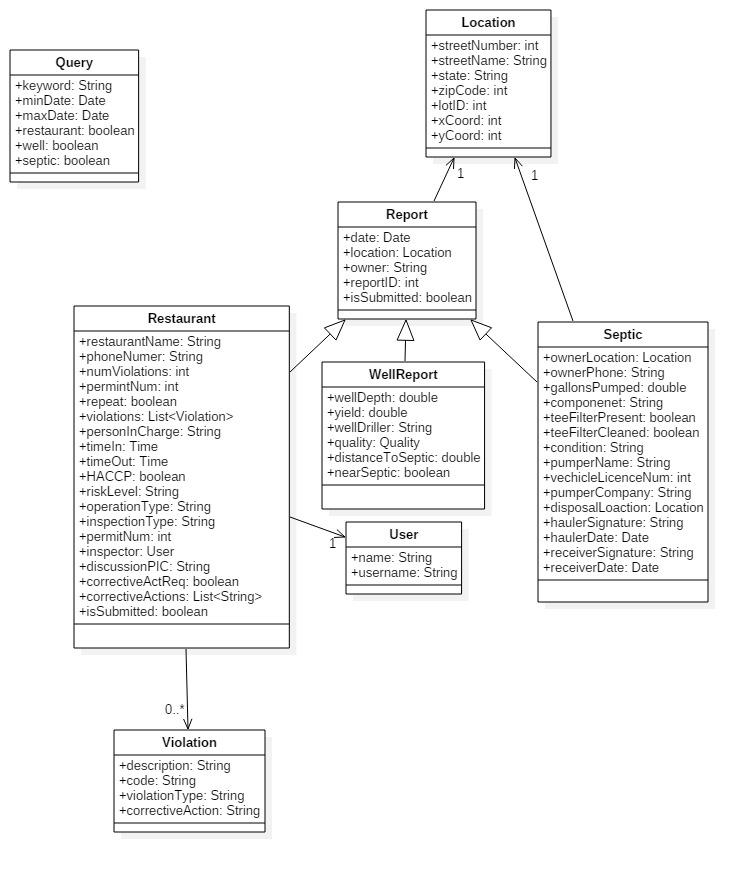
\includegraphics[width=6in,height=6in]{uml.jpg}
\caption{Shows abstractions for data on forms and search.}
\end{figure}

\subsubsection{Delayed Upload}

When control is passed to the DelayedUploadController a few processes can be run. When an update is run locally,

\begin{figure}[H]
\centering
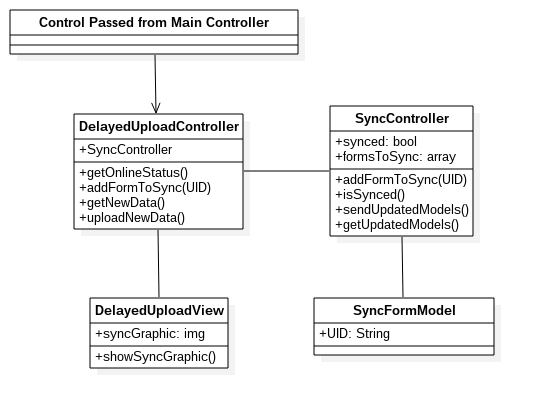
\includegraphics[width=6in,height=6in]{Delayed_Upload_UML.png}
\caption{Shows abstractions for the system's uploading of forms.}
\end{figure}

\subsection[SYSTEM IMPLEMENTATION]{\selectlanguage{english}\rmfamily\bfseries\color{black}
SYSTEM IMPLEMENTATION}
{\selectlanguage{english}\rmfamily\color{black}
All classes and functions described in this section will be written in Javascript. All classes are meant to represent and contain all relevant information pertaining to their real life incarnations. Thus, class attributes for reports are predominantly taken from official documents, and all supporting classes utilize as much real-world information as is relevant.
\subsubsection{Class Definitions}
\begin{itemize}
\item restaurant - contains basic information on the restaurant
\item report - Superclass for restaurantReport, wellReport and SepticReport classes. Contains most basic report/form information.
\item restaurantReport - Subclass of report. contains information on restaurants that pertain to the restaurant inspections.
\item wellReport -  Subclass of report. Contains all fields pertaining to Well Report input.
\item septicReport - Subclass of report. Contains all fields pertaining to Septic Report input.
\item location - Specific information pertaining on where to find a specific location .
\item user - References the user/inspector that is logged into the system and submitting a restaurant report.
\item violation - Specifics to the type of restaurant violation including a text description.
\item query - Contains ability to search for past submitted forms by report type, date, and keywords.
\item date - uses the default date class from JavaScript.
\item delayedUploadController - Contains ability to get online status, choose form to sync, get new data, and upload new data.
\item delayedUploadView - Displays the sync graphic when syncing.
\item syncController - Contains ability to check if synced, send updated models, and receive updated models.
\item syncFormModel - Receives the unique identification number.
\end{itemize}
\subsubsection{Function Descriptions}
All classes will have getter and setter methods to give access to the many variables. These functions will be public so information about the reports can be accessed anywhere. Examples include:
\begin{center}
\begin{verbatim}
function isValid?: checks the report to ensure that it is valid to be saved. If it is not, highlights
all invalid inputs.
function submit: allocates memory for the report and saves it to the local database.
function filterRecordsWithQuery(Query query): Given a query, filter the records to show all records
that conform to the query.
function displayRecordWithID(int id): Given a report ID, display the report associated with that ID.
function getRecordsForBrowse(int recordType, String town): Returns all reports of the given type
for the given town.
function getOnlineStatus(): Checks to see if device is connected to the internet.
function addFormToSync(UID): Given the UID, places form in queue to be uploaded
function getNewData(): Checks form to get new data.
function uploadNewData(): Uploads any new data to database.
function showSyncGraphic(): Displays the syncing graphic as upload is in progress.
function synced: returns boolean of is synced or not synced.
function isSynced(): Checks to see if form is synced with the database.
function sendUpdatedModels(): Sends the updated models to the database.
function getUpdatedModels(): Requests the updated models from the database.
\end{verbatim}
\end{center}

\clearpage\section[SYSTEM BEHAVIOR]{\selectlanguage{english}\rmfamily\bfseries\color{black}
SYSTEM BEHAVIOR}

\subsection[FORM ENTRY]{\selectlanguage{english}\rmfamily\bfseries\color{black}
FORM ENTRY}
\subsubsection{Principle Action 1}
\subsubsection{Principle Action 2}
\subsubsection{Principle Action 3}

\subsection[BROWSING AND SEARCH]{\selectlanguage{english}\rmfamily\bfseries\color{black}
BROWSING AND SEARCH}
\subsubsection{Principle Action: Browse Records}
To browse records, the main controller accesses the database for all stored records. The database returns the records, and they are stored in Report objects which are displayed as icons for the user.
\begin{figure}[H]
\centering
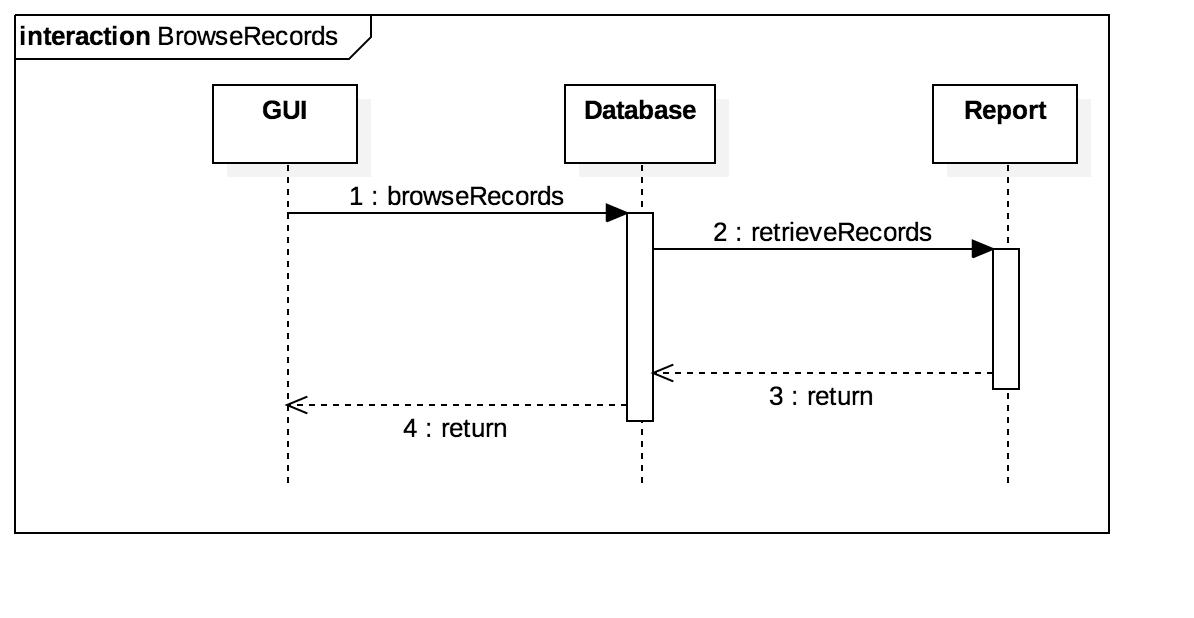
\includegraphics[width=4in,height=2in]{BrowseRecords.png}
\caption{Sequence diagram for retrieving reports for browsing}
\end{figure}
\subsubsection{Principle Action: Search for Reports}
To search for a report, a query object is created from a search string inputted by the user. Through an Ionic plugin, the query filters out the previously loaded reports that are not relevant according to the query string.
\begin{figure}[H]
\centering
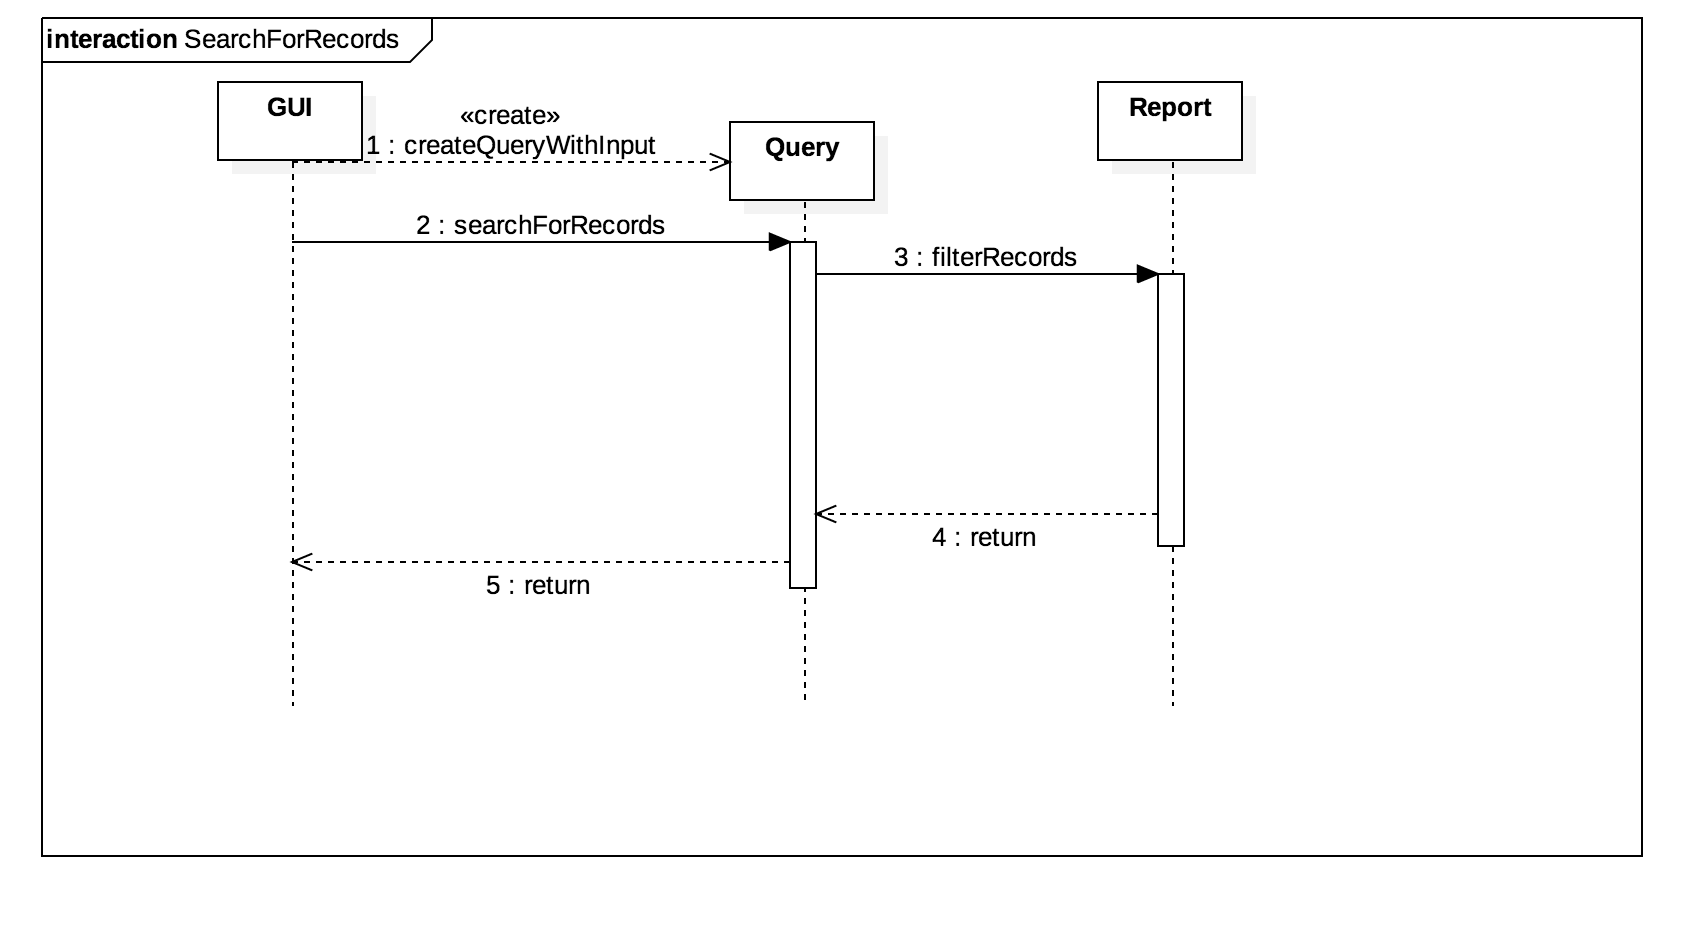
\includegraphics[width=4in,height=3in]{SearchForRecords.png}
\caption{Sequence diagram for filtering stored reports}
\end{figure}
\subsection[DELAYED UPLOAD]{\selectlanguage{english}\rmfamily\bfseries\color{black}
DELAYED UPLOAD}
\subsubsection{Principle Action: Add Document to be Uploaded}
To add a document to be uploaded, control is passed from the main controller to the DelayedUploadController where .addFormToSync is called, thus passing control to the SyncController where the document is added to a queue.
\begin{figure}[H]
\centering
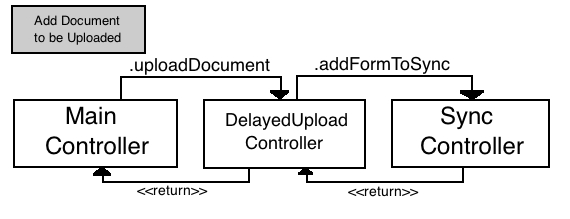
\includegraphics[width=4in,height=2in]{Add.jpg}
\caption{Sequence diagram for adding a document to be uploaded.}
\end{figure}
\subsubsection{Principle Action: Upload Document}
To upload a document, control starts with the SyncController and is passed to the SyncFormModel. The document is then uploaded to the database and the SyncController informs the DelayedUploadController of its success. The DelayedUploadController then updates the status icon for that document using DelayedUploadView.
\begin{figure}[H]
\centering
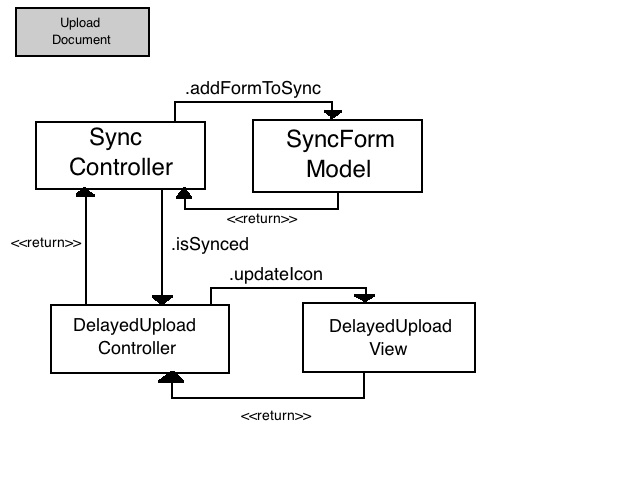
\includegraphics[width=5in,height=3in]{Upload.jpg}
\caption{Sequence diagram for uploading a document.}
\end{figure}


\clearpage\section[DATA DESIGN]{\selectlanguage{english}\rmfamily\bfseries\color{black}
DATA DESIGN}

\clearpage\section[USER INTERFACE DESIGN]{\selectlanguage{english}\rmfamily\bfseries\color{black}
USER INTERFACE DESIGN}

\subsection[DESCRIPTION OF THE USER INTERFACE]{\selectlanguage{english}\rmfamily\bfseries\color{black}
DESCRIPTION OF THE USER INTERFACE}
{\selectlanguage{english}\rmfamily\color{black}
The user interface will consist of various menus through which the user can interact with the tablet application. These menus will include a ''Browsing and Search'' menu, a ''Form Entry'' menu, and a ''Delayed Upload'' status bar. Each menu will contain fields for navigating and performing a specified task. The user will interact with the menus through the device's touch screen.
\newline

\noindent Each menu will consist of various GUI components, such as buttons, labels, text fields, and scroll wheels. These components will be arranged in such a way that the user will be able to quickly navigate through each menu, complete forms, search and browse through the database.
The top of the tablet screen will have a header including an ''add new'' button, a search icon, and a drop down menu. The drop down menu will show options for logging out or sorting the thumbnails on the screen.
\newline

\noindent A detailed description of these menus and their interactions with one another will be described in the following section.
}
\newpage
\subsection[SCREEN OBJECTS \& ACTIONS]{\selectlanguage{english}\rmfamily\bfseries\color{black}
SCREEN OBJECTS \& ACTIONS}
\subsubsection[Browsing and Search]{\selectlanguage{english}\rmfamily\bfseries\color{black}
Browsing and Search}
Upon entering the browsing and search menu, a search text or icon will always be available at the header. When tapped, the search bar will expand and a touch keyboard will appear. The search results will display the search terms and the surrounding text will be displayed along with the search terms. The search terms will be in highlighted in bold font.
\newline

\noindent This design for the search results is influenced by Google's search results pages. Any information that appears next to the search terms may be relevant information that may be accessed without having to open up the full inspection form.
\newline

\noindent The search will also provide suggestions as the user types out the term. There will be an option to sort by category specifically or a date. When the user selects a form that they have found, options to view, edit, email, and print will appear.
\newline

\begin{figure}[h]
\centering
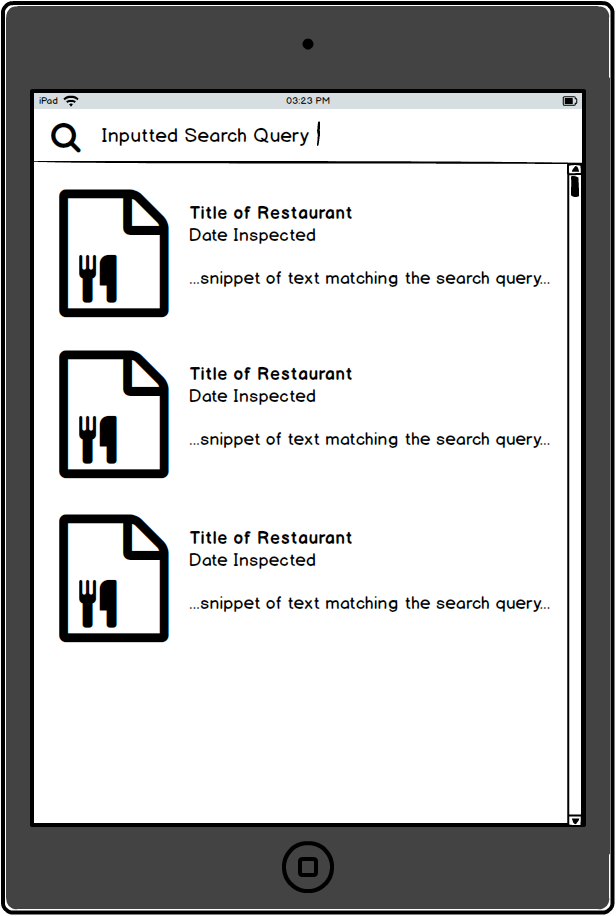
\includegraphics[width=3.5in,height=5in]{Search.png}
\caption{Search screen}
\end{figure}
\newpage
\noindent Three categories will be arranged underneath the header. These categories are restaurants, wells, and septic tanks. A row of documents will present each of these categories and each one will have its own scroll bar. Each document is represented by a thumbnail and will be sorted by most recent starting from left to right.
\newline

\noindent This design for browsing is inspired by Netflix's browsing menus on both their website and mobile applications. The user is greeted with the most recent information entered into the tablet database and shows documents from all three categories of the project. Thumbnail icons are a great way to show the type of documents and any vital information about that document.
\newline

\begin{figure}
    \centering
    \begin{subfigure}[h]{0.4\textwidth}
       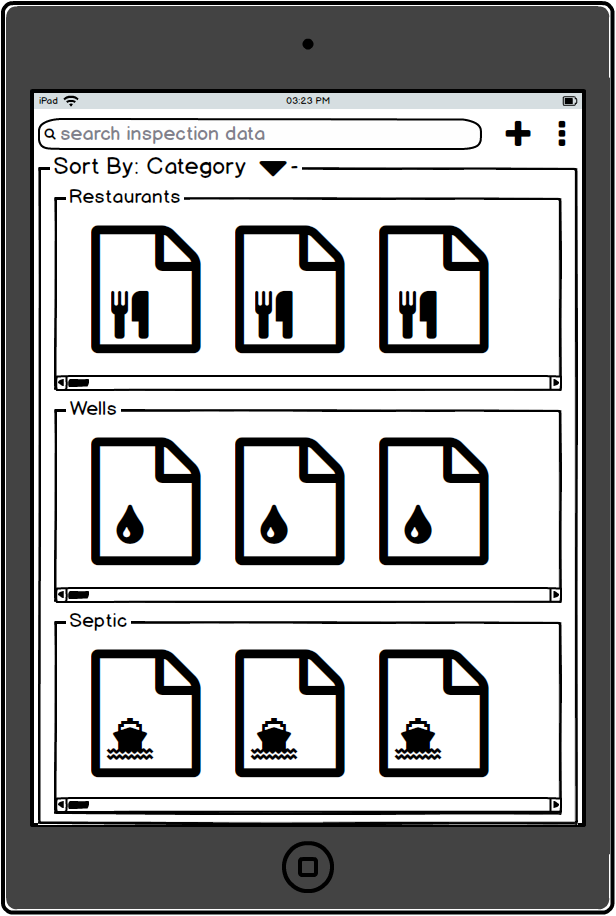
\includegraphics[width=2.5in,height=4in]{Browse_By_Category.png}
    \end{subfigure}
    \qquad
    \begin{subfigure}[h]{0.4\textwidth}
       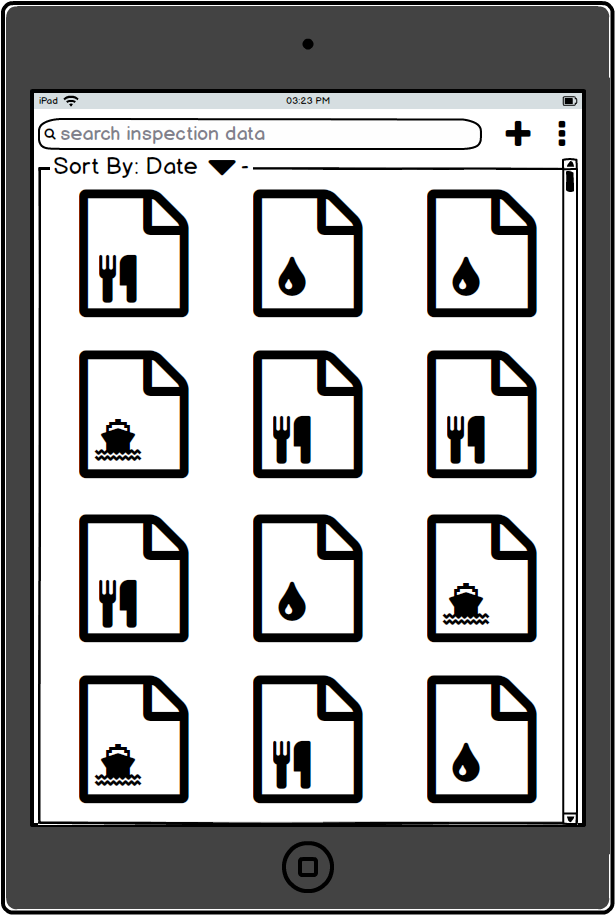
\includegraphics[width=2.5in,height=4in]{Browse_By_Date.png}
    \end{subfigure}
     \caption{Browse by category/date screens}
\end{figure}
\newpage
\noindent When the user taps on one of the three rows of categories, it expands the tapped category to the full screen and displays all of the document thumbnails in that category. The document thumbnails are sorted by most recent starting left to right while going top to bottom. The user can scroll vertically to view more document thumbnails. A user can tap on a thumbnail on the screen and options to view, edit, email, and print will be displayed.
\newline

\noindent This option for browsing may be a quicker way to find documents since it filters by document type to start and displays more thumbnails on the screen at once compared to the rows that are displayed by default.
\newline

\begin{figure}[H]
\centering
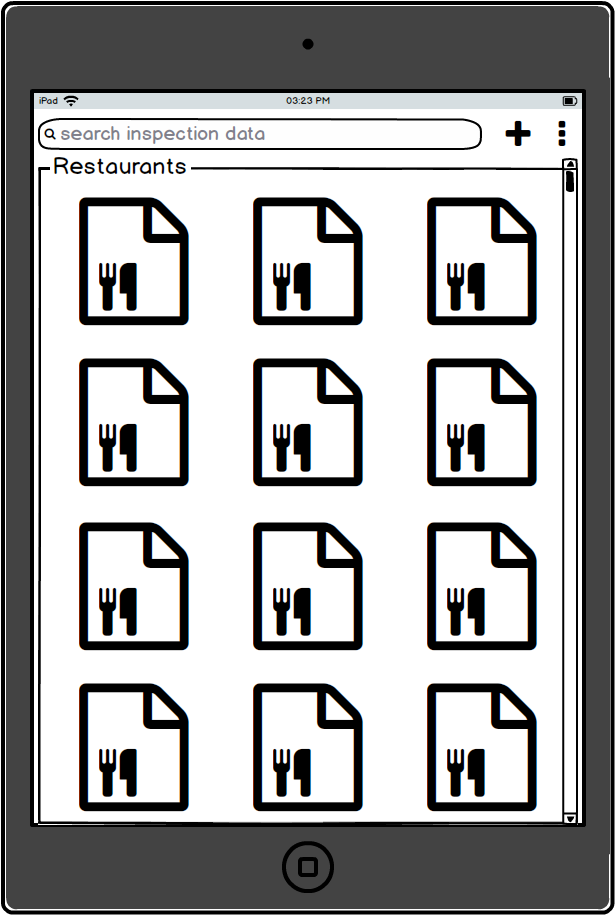
\includegraphics[width=3.5in,height=5in]{Specific_Category_Restaurants.png}
\caption{Specific category chosen screen}
\end{figure}
\newpage

\subsubsection[Form Entry]{\selectlanguage{english}\rmfamily\bfseries\color{black}
Form Entry}
Upon choosing a form, the tablet displays a simple blank form with fillable text fields (see Figure 6). For the restaurant inspection form, information is split into different sections. Each section will be color coded similarly to the paper form currently used.
\newline

\noindent When a field is tapped, the tablet's on-screen touch keyboard will appear. The whole fillable form is displayed on one screen and the user will scroll vertically.
\newline

\noindent A ''complete'' button will be shown on the tablet screen. When the button is tapped, the data entered will be applied to a PDF form and several buttons including print, edit, email, and exit will appear on the screen. A sync status will also appear here.

\begin{figure}
    \centering
    \begin{subfigure}[H]{0.4\textwidth}
  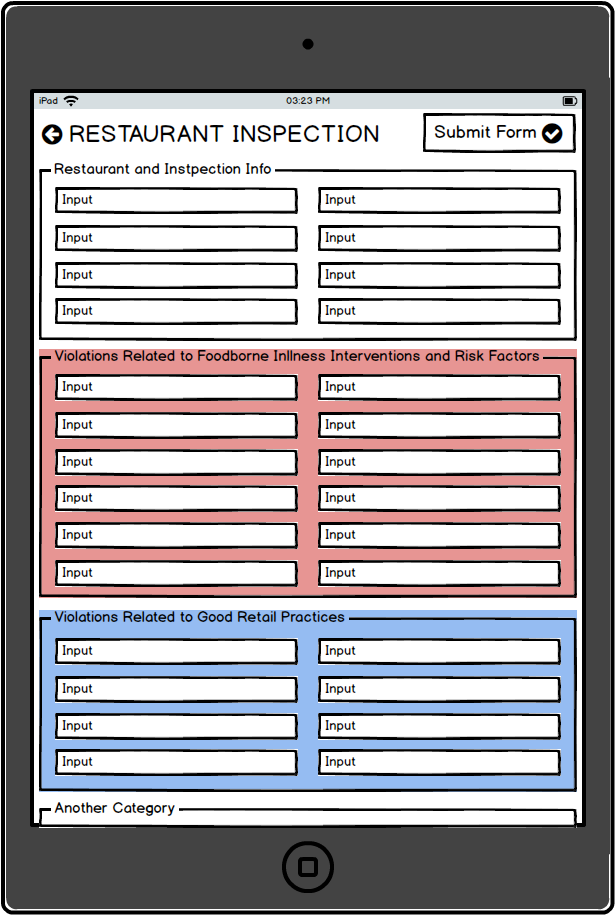
\includegraphics[width=2.5in,height=4in]{Restaurant_Data_Entry_Form.png}
    \end{subfigure}
    \qquad
    \begin{subfigure}[H]{0.4\textwidth}
  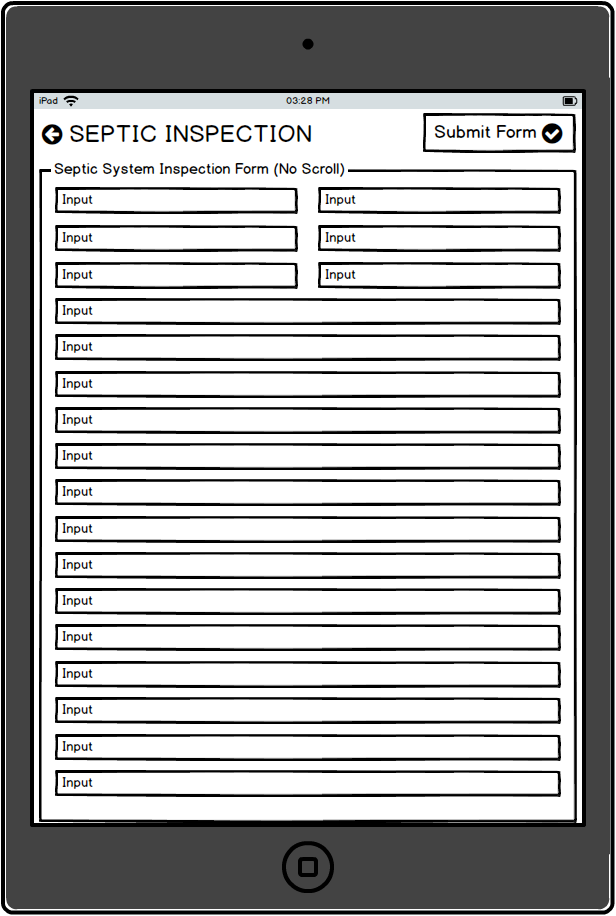
\includegraphics[width=2.5in,height=4in]{Septic_Data_Entry_Form.png}
    \end{subfigure}
     \caption{Restaurant Inspection/Septic Report screens}
\end{figure}

\newpage
\subsubsection[Delayed Upload]{\selectlanguage{english}\rmfamily\bfseries\color{black}
Delayed Upload}
There will be 2 different icons shown on each document thumbnail. Each of these icons will have a distinctive shape and color. A blue sync icon means an upload is in progress. A red sync icon means upload has failed and will try again when network is available. No icon means the file is successfully on the server.
\newline

\noindent The auto-hiding status bar at the bottom of the screen appears when syncing (blue) or when syncing has failed (red) and will be hidden when there is nothing to be synced.
\begin{figure}
    \centering
    \begin{subfigure}[t]{0.4\textwidth}
  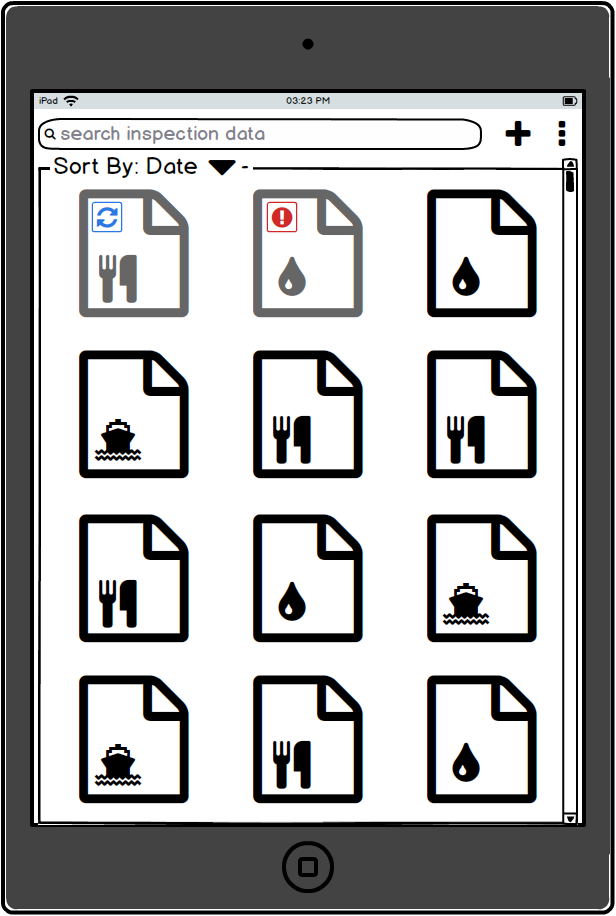
\includegraphics[width=2.5in,height=4in]{Delayed_Upload_Main_Screen.png}
  \caption{Sync icons}
    \end{subfigure}
    \qquad
    \begin{subfigure}[t]{0.4\textwidth}
  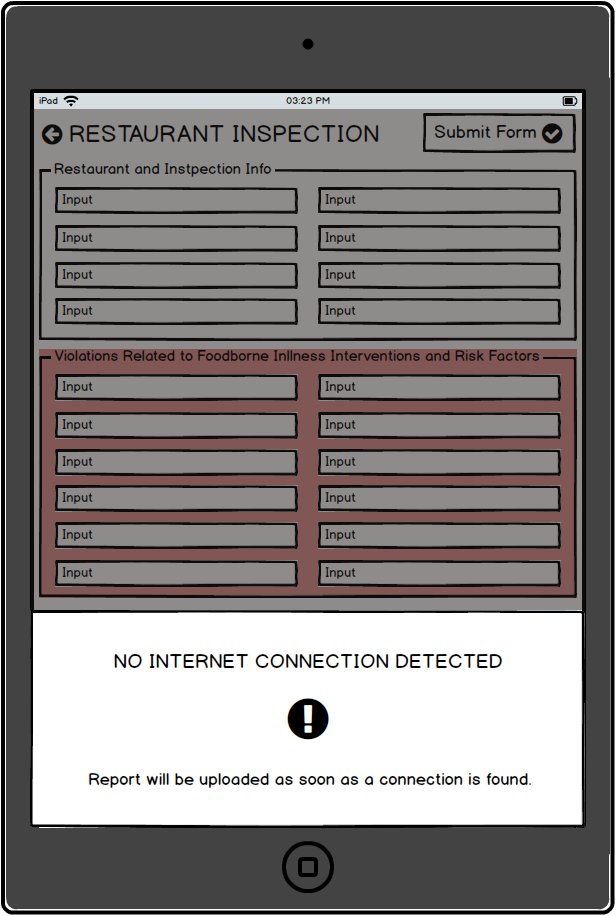
\includegraphics[width=2.5in,height=4in]{Delayed_Upload_Modal.png}
    \caption{Submitting form with no internet access}
    \end{subfigure}
    \caption{Delayed Upload Screens}
\end{figure}
\end{document}
